\section{Durchführung}

\begin{figure}
    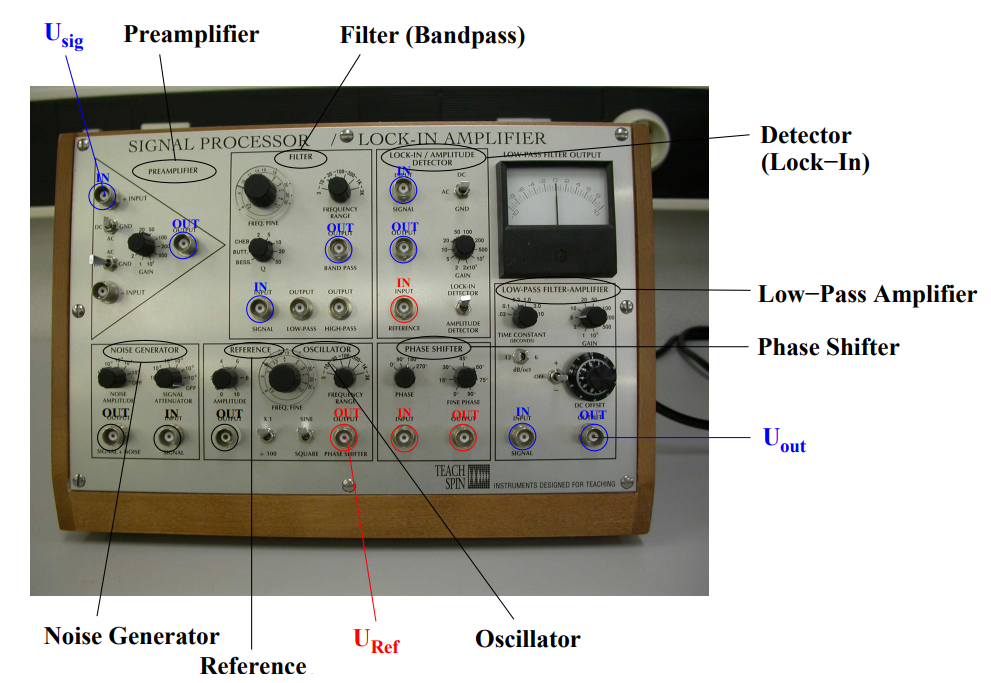
\includegraphics[width=\textwidth]{Abbildungen/Aufbau.png}
    \caption{Der Schematische Aufbau des Lock-In-Verstärkers \cite[][]{man:v303}}
    \label{fig:Lock-In-Bild}
\end{figure}
Ein Lock-In-Verstärker wie in Abb. \ref{fig:Lock-In-Bild} dargestellt wird aufgebaut.
Es werden die Signale des Funktionsgenerators (Reference und Oscillator) mit einem Oszilloskop gemessen \cite[][]{man:v303}.

\subsection{Messungen mit und ohne Störsignal}
\begin{figure}
    \includegraphics[width=\textwidth]{Abbildungen/Schaltplan-Lock-In-Verstärker.png}
    \caption{Der Schematische Aufbau des Lock-In-Verstärkers \cite[][]{man:v303}}
    \label{fig:Lock-In-Schema}
\end{figure}
Die Verbindungen werden wie in Abb. \ref{fig:Lock-In-Schema} nachgebaut.
Um die grundlegene Funktion ohne Störung zu demonstrieren wird der Noise-Generator überbrückt,
d.h. der Pre-Amplifier wird direkt mit dem Reference Ausgang des Funktionengenerators verbunden.
Dieser wird auf eine Frequenz von $\qty[]{1}{\kilo\hertz}$ und eine Amplitude von $\qty{10}{\milli\volt}$ eingestellt.
Der Bandpassfilter wird auf die gleiche Frequenz eingestellt.
Die Einstellungen der Verstärker im Preamplifier und im Lock-In/Amplitude Detector (vgl. \ref{fig:Lock-In-Bild}) werden notiert. 
Das Oszilloskop wird an den Ausgang \enquote{Lock-in / Amplitude Detector} angeschlossen.
An diesem Ort wird die Mischung von $U_\text{ref}$  und $U_\text{sig}$ ausgelesen.
Mithilfe des Speicher-Funktion des Oszilloskops werden Messungen für 5 verschiedene Phasenunterschiede aufgenommen.
% Hier vielleicht ein neuer Absatz (Hihi)
Im nächsten Schritt wird der zweite Kanal des Oszilloskops an den Ausgang des Tiefpasses angeschlossen.
Die Zeit über die der Tiefpass integriert wird mit der Einstellung \enquote{Time-Constant} ausgewählt. 
Sie sollte größer sein als eine Umlaufdauer von $\omega$ damit alle Oberschwingungen aus $U_\text{out}$ herausgefiltert werden.
In dieser Konfiguration werden 10 unterschiedliche Phasenverschiebungen mit dem Oszilloskop aufgenommen.
%
Schließlich wird noch der Rauschgenerator zwischen die Sinusschwingung und den Lock-In-Verstärker geschaltet.
Die Stärke des Rauschens wird auf die gleiche Größenordnung wie die Amplitude von $U_\text{sig}$ eingestellt 
und die Messungen werden wiederholt.

\subsection{Messung mit LED}

Das Prinzip des Lock-In-Verstärkers soll als nächstes mit der Messung eines mit Licht übertragenen Signals demonstriert werden.
\begin{figure}
    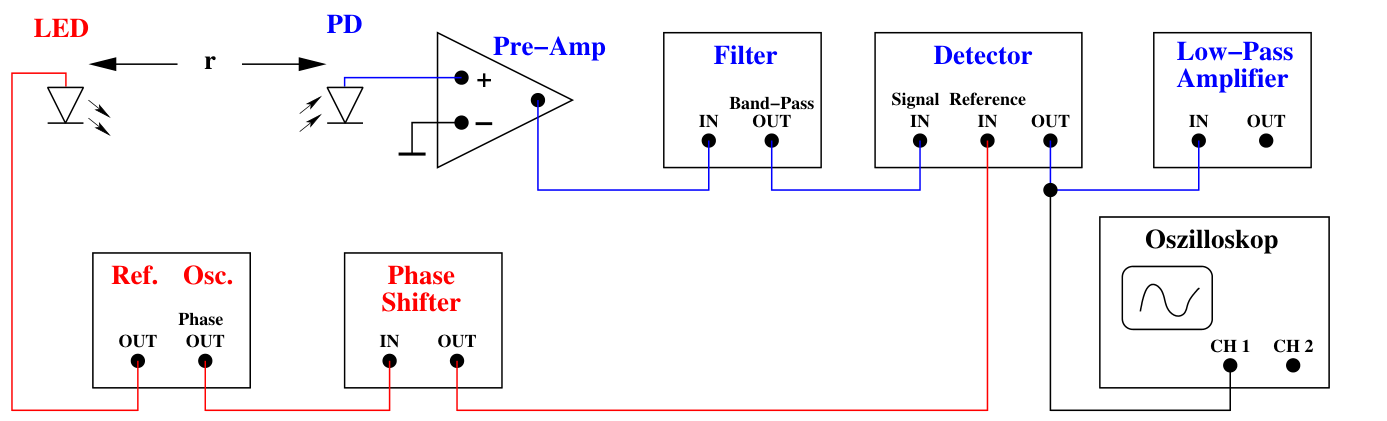
\includegraphics[width=\textwidth]{Abbildungen/Lock-In-mit-LED-Signal.png}
    \caption{Der Lock-In-Verstärker mit einem LED Signal \cite[][]{man:v303}}
    \label{fig:Lock-In-LED}
\end{figure}
%
Hierzu werden eine LED und ein Photodiode wie in Abb. \ref{fig:Lock-In-LED} anstelle des Rauschgenerators eingebaut.
Die LED wird mit einer Rechteckspannung des Funktionsgenerators bei etwa $\qty{200}{\hertz}$ zum Blinken gebracht.
Die genaue Frequenz wird vom Oszilloskop abgelesen. 
Der Abstand $r$ (vgl. Abb. \ref{fig:Lock-In-LED}) wird schrittweise vergrößert und $U_\text{out}$ wird gemessen.
% Der folgende Stz ist vielleicht nicht ganz nötig.
%Auch mit einer großen Menge an Störsignalen aus dem Sonnenlicht und der Raumbeleuchtung sollte ein Signal zu erkennen sein.